\documentclass[blue]{beamer}
\usepackage{beamerthemeFrankfurt} 
\usecolortheme{rose}
\usepackage{amsmath}
\usepackage{amssymb}
%\usepackage{cite} % never use with beamer 
\usepackage{hyperref}
\usepackage{latexsym}
\usepackage{graphicx}
\usepackage{multirow}
\usepackage{adjustbox}
\makeatletter
\newcommand{\removelatexerror}{\let\@latex@error\@gobble}
\makeatother
\makeatletter
\let\@@magyar@captionfix\relax
\makeatother
\usepackage{url}
\newtheorem{assumption}{Assumption}
\usepackage{setspace}
\setbeamertemplate{itemize/enumerate body begin}{\small}
\usepackage{tabulary}
\usepackage[algo2e,linesnumbered,ruled,vlined]{algorithm2e} 
%\usepackage{algpseudocode,algorithm,algorithmicx}
\setbeamercolor{title}{fg=red!80!black,bg=red!20!white}
 %   \setbeamerfont{block title}{size=\scriptsize} change block title font size
%\setbeamerfont{title}{shape=\itshape,family=\rmfamily}
%\usetheme{Warsaw} % brings shadowness
\usefonttheme{professionalfonts} % font theme
\newtheorem{answeredquestions}[theorem]{Answered Questions}
\usepackage[figuresright]{rotating}
\usepackage{subfig}
\graphicspath{{images/}}
%\usefonttheme[onlysmall]{structurebold} %%%small fonts in the navigation bars are a bit hard

\title{Linear Regression: An Introductory Course}
\author[Chandresh]{Chandresh Kumar Maurya, PhD\\ }
\institute{Assistant Professor in CSE deptt at IIT Indore  }
\begin{document}
\maketitle
% without [fragile], any {verbatim} code gets mysterious errors.



\begin{frame}
\frametitle{Outline}
  \tableofcontents %[pausesections]
\end{frame}
%====================================================
\section{Introduction}

\begin{frame}{An example}
Suppose we have been given some data about how many hours of study you do and it determines the grade or percentage score that
you will get in the final exam. Denote the number of hours studied by ${x}$ and grade or percentage obtained is $y$.

\begin{figure}
\centering
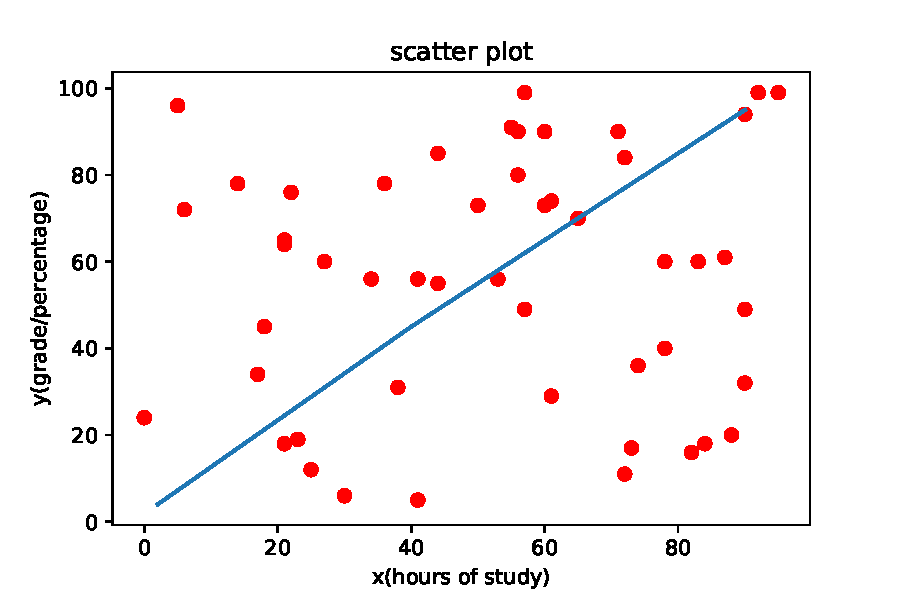
\includegraphics[width=7cm,height=6cm]{lr.pdf}
\caption{A scatter plot of hours of study and grade/percentage}
\label{linear}
\end{figure}
\end{frame}

\begin{frame}{The model}
Our model here is a line which we use to predict $y$ given $x$. Recall the equation of a line from high school geometry class.
\begin{equation}\label{line}
y = mx + c
\end{equation}
Here $x$ is called the \alert{ predictor variable} and $y$ the {\color{blue} response variable}. 
Given $\{x,y\}$ pairs, our objective is to find the line which represents the data in the best possible way.  \\
{\bf The Question}:  what is the best possible way?
\end{frame}

\begin{frame}{The model}
A line which goes through most of the points will be our best line. Next quesstion:\\
How to find such a line? \\

finding a line is to estimate the coefficients $m$ and $c$ in \eqref{line}. \\
How to do that?\\
Recall when we need to find two unknowns, we need two equations at least. \\
\begin{align*}
y_1 = mx_1 +c \\
y_2 = mx_2 +c
\end{align*}
Two equations means we need two data points $(x_1,y_1)$ and $(x_2,y_2)$. This is called simple linear regression in one variable.  A variable is also called \alert{feature}.
\end{frame}

\begin{frame}{The model}
In reality there are more data points and a line should ideally go through all of them. But, this is impossible when all the data points don't lie on the same line. See fig. \ref{linear}. So, what to do in this case?
\begin{figure}
\centering
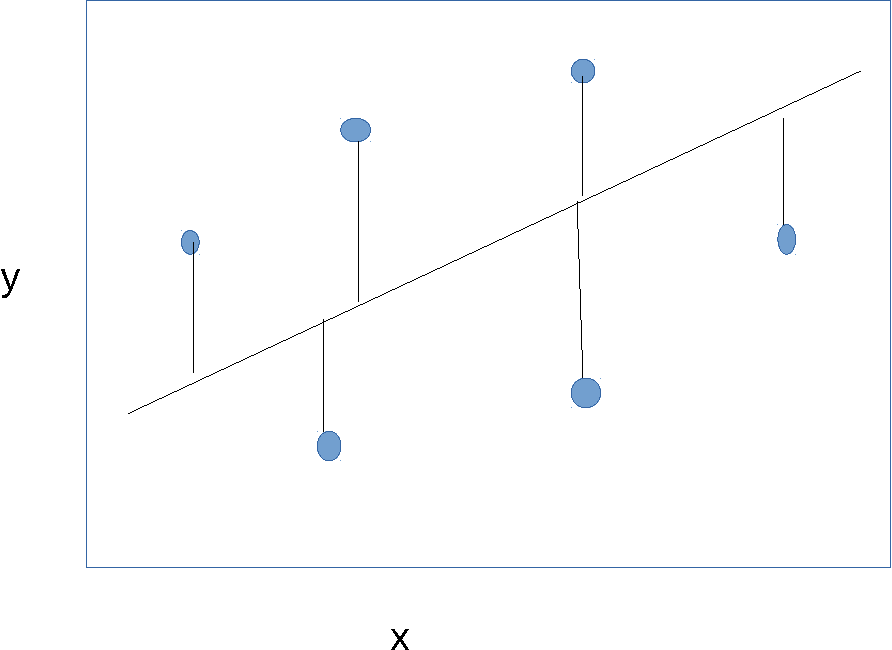
\includegraphics[width=7cm,height=6cm]{error-crop.pdf}
\caption{A scatter plot of hours of study and grade/percentage}
\label{linear}
\end{figure}
\end{frame}
\section{The Objective Function}


\begin{frame}{The Objective function}
Let's say our prediction is $\hat{y}$. So want to minimize the distance $(\hat{y}-y)$.  We have total $n$ data points $\{(x_i,y_i)\}_{i=1}^n$ from which we want to estimate our parameters $(m,c)$ . Hence, we want to minimize the \alert{average squared error} or \alert{mean squared error} (MSE).
\begin{align*}
J(m,c) & =\frac{1}{2n} \sum_{i=1}^n (\hat{y}_i-y_i)^2\\
&=\frac{1}{2n} \sum_{i=1}^n ((mx_i+c)-y_i)^2
\end{align*}
\end{frame}

\section{The Solution}

\begin{frame}{The Solution: Calculus way}
Two solution techniques:
\begin{itemize}
\item Using calculus
\item Using optimization

\end{itemize}
Using calculus, we can differentiate the objective function wrt $m$ and $c$. So, we get
\begin{align*}
m &= \frac{ n\sum_{i=1}^n x_i\sum_{i=1}^ny_i-\sum_{i=1}^n x_iy_i}{n\sum_{i=1}^n x_i^2- (\sum_{i=1}^nx_i)^2} \\
&=\frac{ Cov(X,Y)}{Var(X)} 
\\
c &=\frac{\sum_{i=1}^ny_i -m \sum_{i=1}^n x_i}{n}
\end{align*}
\end{frame}

\begin{frame}{The Solution: Optimization way}
We can use gradient descent to optimize the objective function.
\begin{figure}
\centering
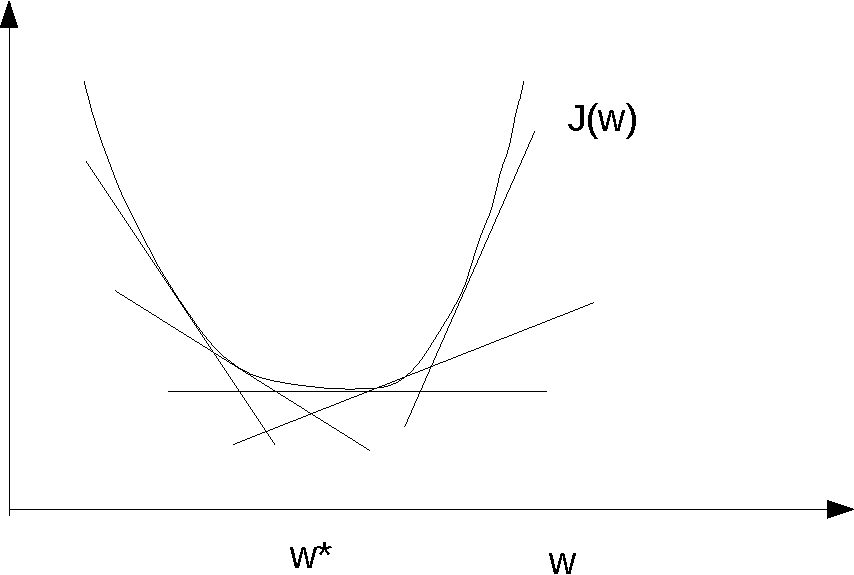
\includegraphics[width=7cm,height=5cm]{gd1-crop.pdf}
\caption{Gradient descent intuition}
\label{linear}
\end{figure}
\end{frame}

\begin{frame}{The Solution: Optimization way}
We can use gradient descent to optimize the objective function.
\begin{figure}
\centering
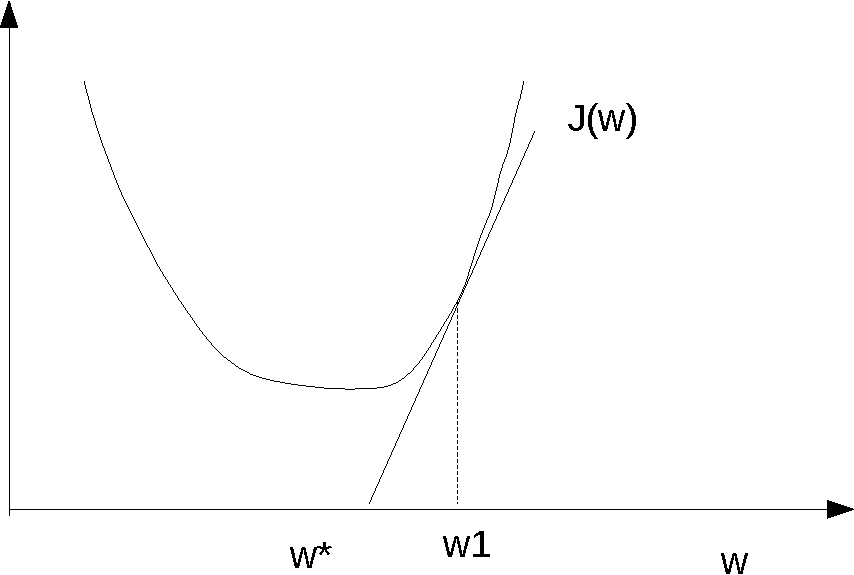
\includegraphics[width=7cm,height=5cm]{linearapprox-crop.pdf}
\caption{Gradient descent intuition}
\label{linear}
\end{figure}
\end{frame}

\begin{frame}{The Solution: Optimization way}
linear approx (infact linear  plus a quadratic term equal to $\frac{L}{2} (w-w_1)^2 ) J(w)$ around $w_1$ can be written as:
\begin{equation} \label{linapprox}
J(w) = J(w_1) + h\nabla J(w_1)
\end{equation}
To minimize \eqref{linapprox}, we can set $h=-\alpha\nabla J(w)$.  To see this, diff \eqref{linapprox} wrt $h$.
Thus update equation for $w$ is given by:
\begin{equation}
w_{t+1}:= w_t-\alpha \nabla J(w)
\end{equation}
$t \in \{1,\ldots,T\}$
\end{frame}
\begin{frame}{The Solution: Gradient Descent}
Large learning rate \alert{$\alpha$} can diverge and overshoot the minimum.
\begin{figure}
\centering
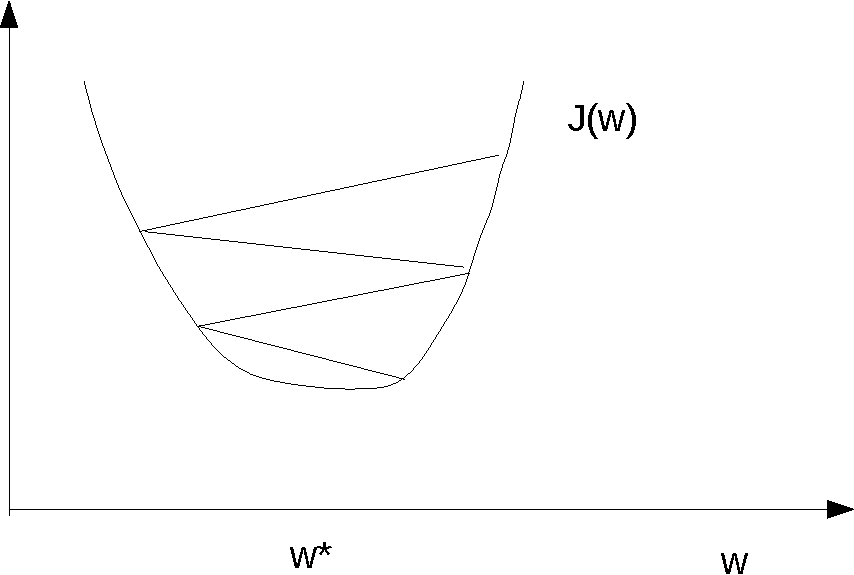
\includegraphics[width=7cm,height=5cm]{largealpha-crop.pdf}
\caption{Gradient descent intuition}
\label{linear}
\end{figure}
\end{frame}

\begin{frame}{The Solution: Gradient Descent}
Small learning rate \alert{$\alpha$} can be too slow to converge.
\begin{figure}
\centering
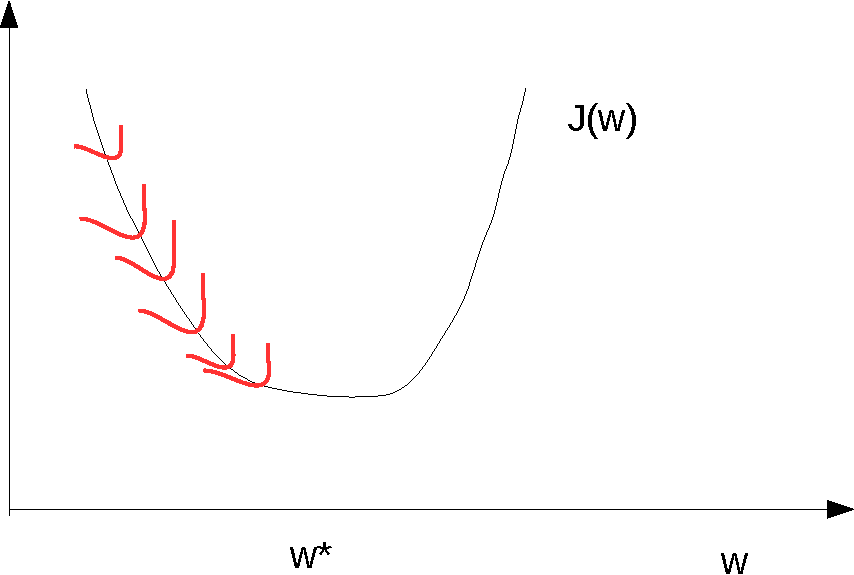
\includegraphics[width=7cm,height=5cm]{smallalpha-crop.pdf}
\caption{Gradient descent intuition}
\label{linear}
\end{figure}
\end{frame}

\begin{frame}[allowframebreaks]{Bibliography}
\fontsize{8pt}{7.2}\selectfont
\bibliographystyle{apalike}
\bibliography{./TKDE}
\end{frame}
\end{document}